\ifdefined\COMPLETE
\else
\documentclass[12pt]{article}
\usepackage{enumitem}
\usepackage{tikz}
\usepackage{amsmath}

\DeclareMathOperator{\avg}{avg}
\usetikzlibrary{shapes, calc, arrows, through, intersections, decorations.pathreplacing, patterns}
\begin{document}
\fi

%\def\alph{$2+\sqrt{5}$}
\begin{figure}
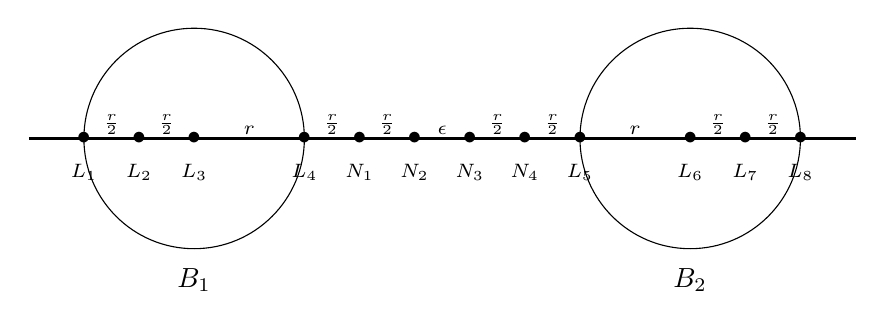
\begin{tikzpicture}[scale=7]

	\coordinate (x) at ($ (-0.1,{sqrt(0)}) $);
	\coordinate (y) at (1.4,0);
	\draw[thick] (x) --(y);

	\node[label=270:$\scriptstyle L_1$] at (0.0,0) {$\bullet$};
	\node[label={[yshift=-0.2cm]\scriptsize $\frac{r}{2}$}] at (0.05,0) {};
	\node[label=below:{$\scriptstyle L_2$}] at (0.1,0) {$\bullet$};
	\node[label={[yshift=-0.2cm]\scriptsize $\frac{r}{2}$}] at (0.15,0) {};
	\node[label=below:{$\scriptstyle L_3$}] at (0.2,0) {$\bullet$};
	\node[label={[yshift=-0.2cm]\scriptsize $r$}] at (0.3,0) {};
	\node[label=270:$\scriptstyle L_4$] at (0.4,0) {$\bullet$};
	
	\node[label={[yshift=-0.2cm]\scriptsize $\frac{r}{2}$}] at (0.45,0) {};
	\node[label=below:{$\scriptstyle N_1$}] at (0.5,0) {$\bullet$};
	\node[label={[yshift=-0.2cm]\scriptsize $\frac{r}{2}$}] at (0.55,0) {};
	
	\node[label=below:{$\scriptstyle N_2$}] at (0.6,0) {$\bullet$};
	\node[label={[yshift=-0.2cm]\scriptsize $\epsilon$}] at (0.65,0) {};
	\node[label=below:{$\scriptstyle N_3$}] at (0.7,0) {$\bullet$};
	
	\node[label={[yshift=-0.2cm]\scriptsize $\frac{r}{2}$}] at (0.75,0) {};
	\node[label=below:{$\scriptstyle N_4$}] at (0.8,0) {$\bullet$};
	\node[label={[yshift=-0.2cm]\scriptsize $\frac{r}{2}$}] at (0.85,0) {};
	
	\node[label=270:$\scriptstyle L_5$] at (0.9,0) {$\bullet$};
	\node[label={[yshift=-0.2cm]\scriptsize $r$}] at (1.0,0) {};
	\node[label=270:$\scriptstyle L_6$] at (1.1,0) {$\bullet$};
	\node[label={[yshift=-0.2cm]\scriptsize $\frac{r}{2}$}] at (1.15,0) {};
	\node[label=below:{$\scriptstyle L_7$}] at (1.2,0) {$\bullet$};
	\node[label={[yshift=-0.2cm]\scriptsize $\frac{r}{2}$}] at (1.25,0) {};
	\node[label=270:$\scriptstyle L_8$] at (1.3,0) {$\bullet$};	
		
	\node[label=270:$B_1$] at (0.2,-0.2) {};	
	%\node[label=270:$B_{12}$] at (0.5,-0.15) {};	
	\node[label=270:$B_2$] at (1.1,-0.2) {};	
	\draw (0.2,0) circle (0.2cm);
	\draw (1.1,0) circle (0.2cm);
\end{tikzpicture}
\caption{Clustering ${B_1, B_2}$ satisfies $(\lambda, \eta)$-center separation for $\lambda > 4$. However, both single-linkage and max-linkage don't work for this example.}
\end{figure}

Let $t$ be some parameter. $t$ points are concentrated at the location $L_i$. The locations $N_i$ contain just a single point. It is easy to see that $C = \{B_1, B_2 \}$ satisfies $(\lambda, \eta)$-center separation for $\lambda \ge 4$ and $\eta \le 1$. It is fairly easy to see that single-linkage on this example will end up merging $L_4, L_5$ together and will split the clusters $B_1$ and $B_2$. Now, let us examine how max-linkage works on this example.

Max-linkage starts with all the points in its own individual cluster. It then merges clusters with smallest $d_{\max}$ where $d_{\max}(A, B) = \max\{d(a, b): a \in A, b \in B\}$. Hence, max linkage on the above example proceeds as follows. 
\begin{itemize}[nolistsep] 
\item $d_{\max} = \epsilon$. $N_2, N_3$ are merged together. 
\vspace{-0.1in}\begin{align*}
C = \{\{L_1\},\{L_2\},\{L_3\},\{L_4\},\{N_1\},\{N_2,N_3\},\{N_4\},\{L_5\},\{L_6\},\{L_7\},\{L_8\}\}
\end{align*}
\item \vspace{-0.1in} $d_{\max} = \frac{r}{2}$. Next, $L_2, L_3$ and $L_6, L_7$ and $L_4, N_1$ and $L_5, N_4$ are merged together. 
\vspace{-0.1in}\begin{align*}
C = \{\{L_1\},\{L_2,L_3\},\{L_4, N_1\},\{N_2,N_3\},\{N_4, L_5\},\{L_6, L_7\},\{L_8\}\}
\end{align*}
\item \vspace{-0.1in} $d_{\max} = r$. Next, $L_1$ and $L_8$ are merged into the corresponding clusters. 
\vspace{-0.3in}\begin{align*}
C = \{\{L_1, L_2,L_3\},\{L_4, N_1\},\{N_2,N_3\},\{N_4, L_5\},\{L_6, L_7, L_8\}\}
\end{align*}
\item \vspace{-0.1in} $d_{\max} = r+\epsilon$. WLOG, the cluster containing $L_4$ is merged with cluster containing $N_3$. 
\vspace{-0.1in}\begin{align*}
C = \{\{L_1, L_2,L_3\},\{L_4, N_1, N_2,N_3\},\{N_4, L_5\},\{L_6, L_7, L_8\}\}
\end{align*}
\item \vspace{-0.1in} $d_{\max} = 2r+\epsilon$. $L_4$ and $L_5$ are merged together. 
\vspace{-0.1in}\begin{align*}
C = \{\{L_1, L_2,L_3\},\{L_4, N_1, N_2,N_3, N_4, L_5\},\{L_6, L_7, L_8\}\}
\end{align*}
\end{itemize}

Hence, we see that in the max-linkage hierarchical clustering tree none of the prunings are laminar with ${B_1, B_2}$. The same example also works for average-linkage. Average-linkage merges clusters with smallest $d_{\avg}$ where $d_{\avg}(A, B) = \frac{\sum_{a \in A, b \in B} d(a, b)}{|A||B|}$. Average-linkage on this example proceeds identical to max-linkage above. For the sake of completeness we will provide the details. For this example, we will fix $t = 2$. 

\begin{itemize}[nolistsep] 
\item $d_{\avg} = \epsilon$. $N_2, N_3$ are merged together. 
\vspace{-0.1in}\begin{align*}
C = \{\{L_1\},\{L_2\},\{L_3\},\{L_4\},\{N_1\},\{N_2,N_3\},\{N_4\},\{L_5\},\{L_6\},\{L_7\},\{L_8\}\}
\end{align*}
\item \vspace{-0.1in} $d_{\avg} = \frac{r}{2}$. Next, $L_2, L_3$ and $L_6, L_7$ and $L_4, N_1$ and $L_5, N_4$ are merged together. 
\vspace{-0.1in}\begin{align*}
C = \{\{L_1\},\{L_2,L_3\},\{L_4, N_1\},\{N_2,N_3\},\{N_4, L_5\},\{L_6, L_7\},\{L_8\}\}
\end{align*}
\item \vspace{-0.1in} $d_{\avg} = \frac{3r}{4}$. Next, $L_1$ and $L_8$ are merged into the corresponding clusters. 
\vspace{-0.3in}\begin{align*}
C = \{\{L_1, L_2,L_3\},\{L_4, N_1\},\{N_2,N_3\},\{N_4, L_5\},\{L_6, L_7, L_8\}\}
\end{align*}
\item \vspace{-0.1in} $d_{\avg} = \frac{5r+3\epsilon}{6}$. WLOG, the cluster containing $L_4$ is merged with cluster containing $N_3$. 
\vspace{-0.1in}\begin{align*}
C = \{\{L_1, L_2,L_3\},\{L_4, N_1, N_2,N_3\},\{N_4, L_5\},\{L_6, L_7, L_8\}\}
\end{align*}
\item \vspace{-0.1in} $d_{\avg} = \frac{20r+12\epsilon}{15}$. Here, we have four clusters $C_1 = \{L_1, L_2,L_3\}$, $C_2 = \{L_4, N_1, N_2,N_3\}$, $C_3 = \{N_4, L_5\}$ and $C_4 = \{L_6, L_7, L_8\}$. Simple calculations show that $d_{\avg}(C_2, C_3) = \frac{20r+12\epsilon}{15}$. However, $d_{\avg}(C_1, C_2) > \frac{3r}{2}$ and $d_{\avg}(C_3, C_4) > \frac{3r}{2}$. Hence, $L_4$ and $L_5$ are merged together.
\vspace{-0.1in}\begin{align*}
C = \{\{L_1, L_2,L_3\},\{L_4, N_1, N_2,N_3, N_4, L_5\},\{L_6, L_7, L_8\}\}
\end{align*}
\end{itemize}

As before, we see that none of the prunings of the average-linkage hierarchical clustering tree are laminar with ${B_1, B_2}$.
\ifdefined\COMPLETE
\else
\end{document}
\fi
